%!TEX root = ../../Master.tex
\section{Organization} % (fold)
\label{sec:organization}


\sinote{Må gerne læses i gennem og kritiseres}

\sinote{Beskriv hvorfor region nord kunne være interreseret i et system der kan adapteres til flere sygehuse. Management time bliver mindre ved dette.}

\sinote{Beskriv at elementer på et hospital ikke altid virker. F.eks. kan en elevator være ude af drift, eller en gang kan være ved at blive malet.}

In order to create a good navigational system for a hospital, certain factors must be considered. When deciding new features for a hospital, installation \& maintenance costs and compatibility with the existing hardware are a big subject. Therefore this section will describe how the existing infrastructure in hospitals is and how this will affect the navigational system.

\subsection{WiFi}

Most hospitals have good WiFi coverage around their cadastral. A visit to \enquote{Sygehus Nord} in Aalborg revealed that multiple locations around the hospital had a sufficient amount of WiFi hotspots in range, in order to be used in Location Based Services. See \cref{fig:wifi1,fig:wifi2,fig:wifi3}.

\begin{figure}
\centering
  \begin{minipage}{0.45\textwidth}
    \centering
    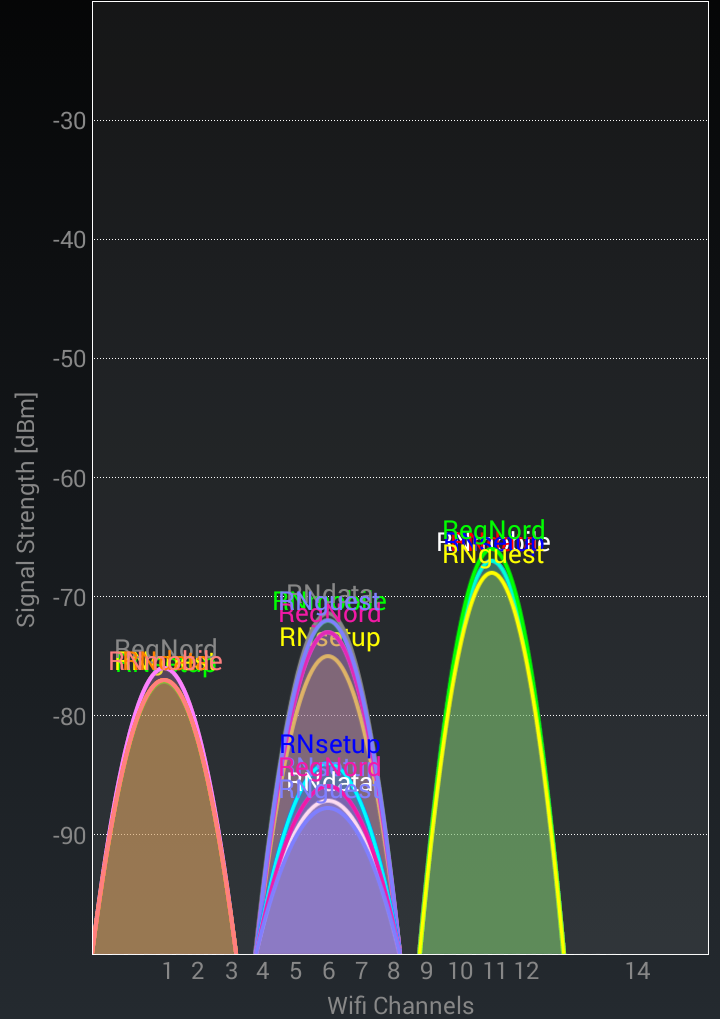
\includegraphics[width=\textwidth]{wifi_sygehus_nord1.png}
    \caption{Graph of signal strength grouped by channels. Location A} \label{fig:wifi1}
  \end{minipage}
  \hfill
  \begin{minipage}{0.45\textwidth}
    \centering
    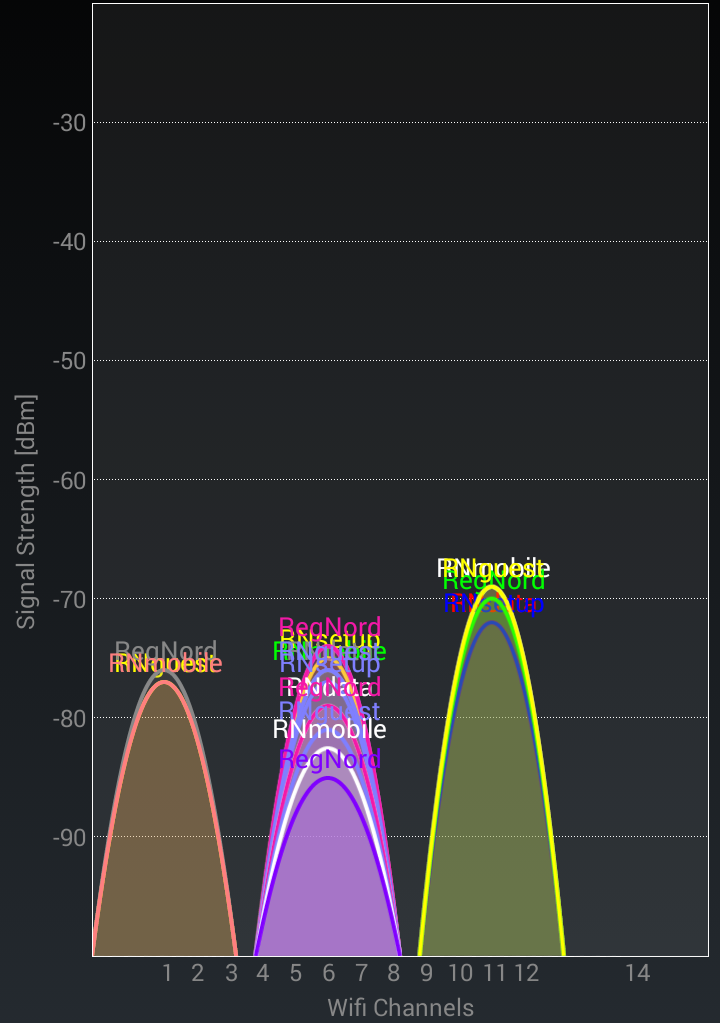
\includegraphics[width=\textwidth]{wifi_sygehus_nord2.png}
    \caption{Graph of signal strength grouped by channels. Location B} \label{fig:wifi2}
  \end{minipage}
    \begin{minipage}{0.45\textwidth}
    \centering
    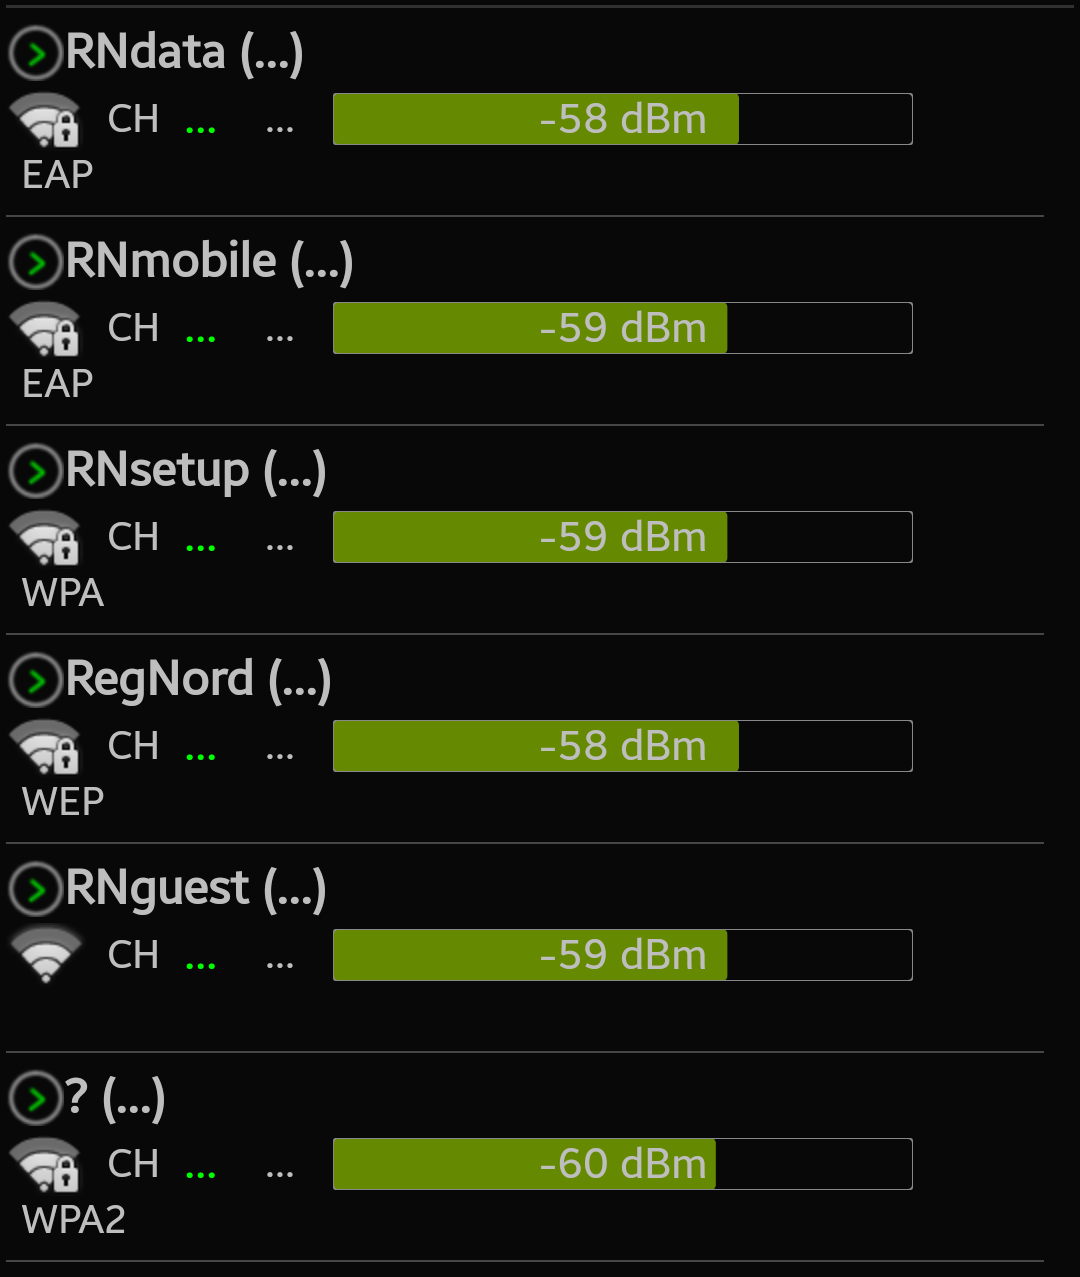
\includegraphics[width=\textwidth]{wifi_sygehus_nord3.png}
    \caption{List of WiFi networks} \label{fig:wifi3}
  \end{minipage}
  \end{figure}


\subsection{Interference with medical device}

Incidents of radio frequency interference between cellular phones, radio broadcasters, WiFi devices and medical devices have been reported. Older models of pacemakers, defibrillators and hearing aid devices were being influenced by near encounter of cellular phones causing undesirable effects like not having control of heartbeat etc.. The problem was that radio frequency fields were interfering with medical equipment. This has however now been addressed in modern standards, meaning that interference with medical devices does not occur any more. \cite{Man1998,Case}

\sinote{Skriv ikke om politik i dette område. Beslutningstagen skal flyttes op i interessenter}

In this section we will cover which procedures are needed in order to realize a software solution for our initiating problem (\cref{sub:init}).

In a decision process the following phases will typically happen. \cite{Sjaelland}

%%\begin{description}
%%	\item[Idea and initiative phase] A problem is defined by the citizens, media or political organisation.
%%	\item[Preparing phase] The problem will be reviewed according to the health legislation.
%%	\item[Decision phase] The problem is presented and a committee is established. This committee will typically work with consultants to specify the requirements of the solution.
%%	\item[Implementation phase] The solution will be implemented. 
%%
%%
%%\end{description}
\begin{itemize}
  \setlength{\itemsep}{1pt}
  \setlength{\parskip}{0pt}
  \setlength{\parsep}{0pt}
	\item \textbf{Idea and initiative phase} A problem is defined by the citizens, media or political organisation.
	\item \textbf{Preparing phase} The problem will be reviewed according to the health legislation.
	\item \textbf{Decision phase} The problem is presented and a committee is established. This committee will typically work with consultants to specify the requirements of the solution.
	\item \textbf{Implementation phase} The solution will be implemented. 
\end{itemize}


Between the decision phase and the implementation phase, the project will be announced as a public supply contract for suppliers to tender. \cite{Union2004}. Suppliers will then submit their solutions. The solution that fits the problem's requirements best, gets the contract. 

% section organization (end)